\section{Macchine di Turing a più nastri}

La descrizione informale della macchina di Turing data nel paragrafo 2 in termini di
nastro, celle e testina è assai elementare, essenziale e schematica, certamente
passibile di adattamenti, modifiche e migliorie. Per esempio, tra le varianti
ammissibili, possiamo considerare l'eventualità di disporre di più nastri di lavoro.
Ma il meccanismo che ne deriva, anche se apparentemente più duttile e potente della
semplice MdT, mantiene in realtà le medesime capacità computazionali: i linguaggi
decisi o accettati restano esattamente gli stessi, così come le funzioni calcolate.
Vediamo perché.\\
Consideriamo allora una macchina di Turing M a più nastri (si veda la figura
sottostante) immaginata come composta da:

\begin{itemize}
    \item una unità di controllo a stati finiti,
    \item un nastro $N_0$ di input-output di lunghezza infinita con relativa testina,
    \item $m$ nastri ausiliari $N_1, \ldots, N_m$ di lunghezza infinita ($m \ge 0$),
          ciascuno dotato di propria testina
\end{itemize}

\begin{figure}[H]
    \centering
    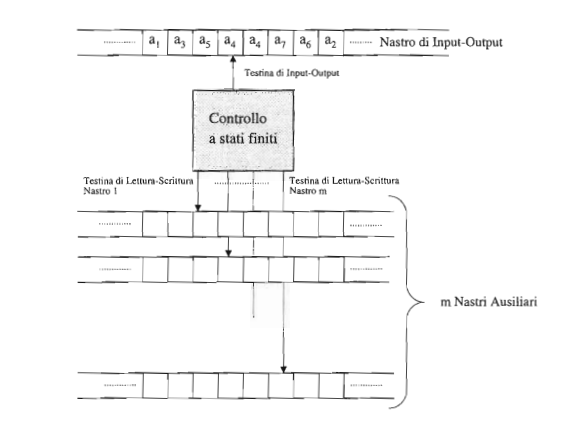
\includegraphics[width=10cm, keepaspectratio]{capitoli/le_macchine_di_turing/imgs/mdt_piu_nastri.png}
    \caption{Schema di una Macchina di Turing a più nastri}
\end{figure}

Ogni nastro è suddiviso in celle, e ogni cella è in grado di memorizzare un simbolo
di un certo alfabeto $A = {a_0, a_1, \ldots, a_n}$, o il simbolo bianco $*$. Il
nastro di input-output $N_0$ contiene l'input iniziale e l'eventuale output finale di
ogni computazione; ma, durante il lavoro, anche gli altri nastri $N_1, \ldots, N_m$
possono
essere coinvolti e adoperati. Ogni nastro è scandito dalla sua testina, secondo le
convenzioni usuali per MdT semplici. L'unità di controllo, oltre a contenere il
programma secondo cui la computazione deve essere eseguita, controlla lo stato della
macchina. All'inizio della computazione, l'input è scritto su $N_0$ e la testina ne
indica il simbolo più a sinistra; gli altri nastri sono vuoti e la testina ne esamina
una cella arbitraria; la macchina $M$ è nello stato $q_0$. Ogni successiva mossa di $M$
è determinata da

\begin{itemize}
    \item il suo stato,
    \item i simboli indicati dalle testine sui vari nastri $N_0, N_1, \ldots, N_m$,
\end{itemize}

e consiste in

\begin{itemize}
    \item aggiornare lo stato,
    \item riscrivere i simboli esaminati su ogni nastro,
    \item spostare in ogni nastro la testina di un passo verso destra o verso
          sinistra.
\end{itemize}

Come già detto, si conviene che l'eventuale output della computazione sia la stringa
scritta in $N_0$ se e quando $M$ si arresta.\\
Tutte le definizioni già date per la MdT
semplice possono essere adattate al nuovo modello, ovviamente con le opportune
modifiche. In particolare, le regole di transizione di una macchina $M$ a $m$ nastri
ausiliari sono fatalmente più elaborate, perché devono tenere conto non solo dello
stato di $M$ e del simbolo indicato su $N_0$, ma anche dei simboli considerati sui
nastri ausiliari $N_1, \ldots, N_m$; la transizione sarà caratterizzata, come detto,
dalla scelta di un nuovo stato e dalle istruzioni di scrittura e spostamento per
ciascun nastro, sia di $N_0$ che di $N_1, \ldots, N_m$. Una regola di transizione
sarà allora della forma

$$
    \delta\left(q, b_0, b_1, \ldots, b_m\right)=\left(q^{\prime}, b^{\prime}_0, x_0, b_1^{\prime}, x_1, \ldots, b_m^{\prime}, x_m\right)
$$

dove:

\begin{itemize}
    \item $q, q^{\prime}$ rappresentano gli stati di $M$ rispettivamente prima e dopo
          la transizione.
    \item per ogni i $\in\{0,1, \ldots, m\}, b_i \in A \cup\{*\}$ è il
          simbolo indicato dalla testina sul nastro $N_i, b^{\prime}_i \in A \cup\{*\}$ il simbolo che
          lo sostituisce, $x_i \in\{-1,+1\}$ lo spostamento che la testina deve compiere.

\end{itemize}

II modello che si ottiene sembra più potente ed espressivo delle semplici MdT.

\paragraph{Esempio.} Vediamo in particolare come una MdT con un nastro ausiliario
$N_1$ sappia controllare, per ogni parola $w=a_{j_1} \ldots a_{j_k}$ su $A$, se
$w=w^{\text {rev }}$ e cioè se
$$
    a_{j_1} a_{j_2} \ldots a_{j_k}=a_{j_k} a_{j_{k-1}} \ldots a_{j_1};
$$
sappia cioè decidere il linguaggio
$$
    \left\{\left(w, w^{r e v}\right) \mid w \in A^*, w=w^{r e v}\right\} .
$$
La computazione di $M$ su un generico $w$ avviene come segue: $M$ inizia il suo
lavoro muovendo simultaneamente la testina di $N_0$ e quella del nastro ausiliario
$N_1$ verso destra, una cella per volta, finchè la testina di $N_0$ non incontra
$*$, cioè termina di leggere $w$. Durante questo movimento, $M$
copia su $N_1$ i simboli letti; quindi $M$ scorre all'indietro $N_1$ e individua il
primo simbolo non bianco. Finalmente, $M$ legge simultaneamente il nastro $N_0$ da
destra a sinistra e $N_1$ da sinistra a destra e controlla che i simboli esaminati
coincidano uno a uno. A seconda dell'esito della verifica scrive $SI$ o $NO$ su $N_0$.\\

Nonostante le apparenze, le capacità computazionali di una MdT a più nastri sono le
stesse di quelle a un solo nastro, come adesso proviamo.

\paragraph{Teorema 2.10.1} \textit{Per ogni $MdT \ M = (Q, A, \delta, q_0)$ a $m$
    nastri ausiliari, esiste una $MdT \ M^{\prime} = (Q^{\prime}, A^{\prime}, \delta^{\prime},
        q_0)$ con $A \supseteq A^{\prime}$ tale che:}
\textit{\begin{itemize}
        \item per ogni linguaggio $L$ su $A$, $L$ è accettato o deciso da $M$
              se e solo se lo è da $M^{\prime}$
        \item per ogni funzione $f$ su stringhe in $A^{\star}$, $f$ è calcolata
              da $M$ se e solo se lo è da $M^{\prime}$
    \end{itemize}
}

\textit{Dimostrazione}.
Dobbiamo simulare il comportamento di $M$ con una MdT "tradizionale" $M^{\prime}$,
nel senso che, per ogni $w \in A^{\star}$,

\begin{enumerate}
    \item se $M \downarrow w$, allora $M^{\prime} \downarrow w$ e $M, M^{\prime}$
          hanno lo stesso output su $w$;
    \item se $M \uparrow w$, allora $M^{\prime} \uparrow w$.
\end{enumerate}

Suddividiamo allora l'unico nastro di $M^{\prime}$ in $2 m+2$ tracce consecutive
$$
    N_0^{\prime}, N_1^{\prime}, \ldots, N_m^{\prime}, N_0^{\prime \prime}, N_1^{\prime \prime}, \ldots, N_m^{\prime \prime} \text {. }
$$
Un nuovo simbolo $\Delta$ nell'alfabeto serve a separarle, segnalando inizio e fine
di ognuna; un ulteriore simbolo $\nabla$ delimita a sinistra e a destra la sequenza
delle tracce. Per ogni $i=0,1, \ldots, m$, le tracce $N_i^{\prime}, N_i^{\prime
    \prime}$ corrispondono al nastro $N_i$ di $M$, in particolare

\begin{itemize}
    \item $N_i^{\prime}$ ne ricopia il contenuto significativo (cioè non vuoto),
    \item $N_i^{\prime \prime}$ provvede a indicare la posizione della testina di
          $N_i$.
\end{itemize}

A quest'ultimo proposito, ammettiamo che $A^{\prime}$ includa due ulteriori simboli
$+,-$ e conveniamo che la cella di $N_i^{\prime \prime}$ corrispondente a quella
indicata dalla testina di $N_i$ contenga $+$, le altre $-$. Per esempio, se
$N_i^{\prime}$ contiene la stringa $a_0 a_1 a_0 a_2$ e la testina indica $a_1,
    N_i^{\prime}$ presenta $a_0 a_1 a_0 a_2$ e $N_i^{\prime \prime}-+--$. Naturalmente il
numero delle celle nella traccia $N_i^{\prime}$ è lo stesso che in $N_i^{\prime
    \prime}$, ma questo comune valore può variare durante la computazione in ragione dei
movimenti di $M$ su $N$ : i delimitatori $\triangle, \nabla$ possono però spostarsi e
segnalare con chiarezza i confini. All'inizio della computazione su un dato input
$w$, il nastro di $M^{\prime}$ si presenta allora nel seguente modo:

\begin{itemize}
    \item $N_0^{\prime}$ contiene $w, N_0^{\prime \prime}$ ha + nella prima cella, -
          nelle altre;
    \item  per $i=1, \ldots, m, N_i^{\prime}$ è bianca, cioè contiene $\star,
              N_i^{\prime \prime}$ ha $+$ nella prima cella e $-$ in tutte le altre.
\end{itemize}

A questo punto $M^{\prime}$ può iniziare la simulazione delle macchine $M$. Ad ogni
regola di transizione di $M$
$$
    \delta\left(q, b_0, b_1, \ldots, b_m\right)=\left(q^{\prime}, b_0^{\prime}, x_0, b_1^{\prime}, x_1, . ., b_m^{\prime}, x_m\right)
$$
$M^{\prime}$ fa corrispondere le istruzioni adeguate a svolgere il seguente lavoro:

\begin{itemize}
    \item $M^{\prime}$ entra nello stato $q^{\prime}$;
    \item per ogni $i=1, \ldots, m, M^{\prime}$ sostituisce $b_i$ con $b_i^{\prime}$
          su $N_i^{\prime}$, e registra lo spostamento $x_i$ su $N_i^{\prime \prime}$ con
          l'uso appropriato $\mathrm{di}+\mathrm{e}-$.
\end{itemize}

Quando $M$ converge, $M^{\prime}$ opera una opportuna pulizia del nastro lasciando
solo il contenuto di $N_0^{\prime}$. Ovviamente questa descrizione del comportamento
di $M^{\prime}$ è forzatamente imprecisa. Le operazioni sopra descritte
necessiterebbero di una implementazione in termini di quintuple secondo quanto
richiesto da una MdT tradizionale. Ma, con un minimo di pazienza, il discorso può
essere precisato. In conclusione $M^{\prime}$ simula adeguatamente il comportamento di $M$, e
corrisponde alle richieste dell'enunciato del teorema.\\

Viceversa, ogni MdT tradizionale può essere facilmente intesa come MdT a più nastri
(che in realtà non ha bisogno di ricorrere ai nastri ausiliari). Dunque i due
modelli, con o senza nastri ausiliari, si rivelano equivalenti.